%\documentclass[dvipdfmx]{beamer}
\documentclass{beamer}                   % lualatex の場合
\usepackage{mySld}

\begin{document}
\title[主記憶]{オペレーティングシステム\\第10章 メモリ管理の実装例}
\date{}

\begin{frame}
  \titlepage
\end{frame}

%\section{}
%=========================================================================
%\begin{frame}
%  \frametitle{}
%\end{frame}

\section{メモリ管理の実装例}
%=========================================================================
\begin{frame}
  \frametitle{メモリ管理の実装例}
  TacOSのメモリ管理プログラムを実装例とする.
  \begin{itemize}
  \item 可変区画方式
  \item ファーストフィット
  \item OSがユーザプロセス領域の割当てに使用
  \item プロセスがヒープ領域を管理するプログラムも同じアルゴリズム
  \end{itemize}
\end{frame}

%=========================================================================
\begin{frame}
  \frametitle{データ構造の初期化}
  \lstinputlisting{Lst/memBlk.cmm}
  \begin{itemize}
  \item {\tt memInit()}はカーネル起動時に一度だけ実行される.
  \item 番兵付きのリストで管理する.
  \end{itemize}
\end{frame}

%=========================================================================
\begin{frame}
  \frametitle{初期化直後のデータ構造}
  \begin{center}
    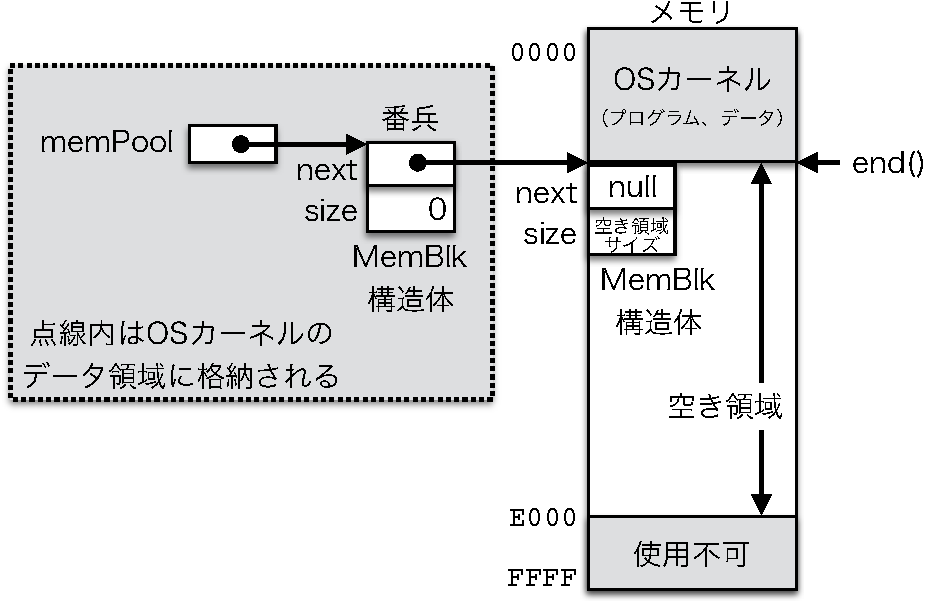
\includegraphics[scale=0.6]{Fig/mmInit-crop.pdf}\\
  \end{center}
  \begin{itemize}
  \item {\tt \_end()}はカーネルサイズにより決まる.
  \item EOOO より後ろはビデオメモリやIPL ROMがある.
  \end{itemize}
\end{frame}

%=========================================================================
\begin{frame}[fragile]
  \frametitle{メモリの割付け}
  右のプログラムでa,b,cを割付けたときのデータ構造
  \begin{center}
    \begin{minipage}{0.39\columnwidth}
    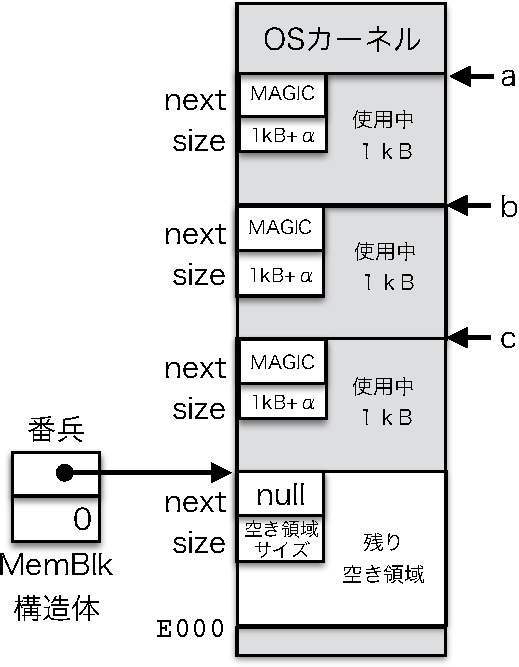
\includegraphics[scale=0.5]{Fig/mmAlloc-crop.pdf}
    \end{minipage}
    \begin{minipage}{0.59\columnwidth}
      \begin{lstlisting}
a = mmAlloc( 1024 );  // 1KiB の領域を割り付ける
b = mmAlloc( 1024 );  // 1KiB の領域を割り付ける
c = mmAlloc( 1024 );  // 1KiB の領域を割り付ける
      \end{lstlisting}
    \end{minipage}
  \end{center}
\end{frame}

%=========================================================================
\begin{frame}
  \frametitle{メモリの割付けプログラム}
  \lstinputlisting[basicstyle={\tiny\ttfamily}]{Lst/mmAlloc.cmm}
\end{frame}

%=========================================================================
\begin{frame}
  \frametitle{領域の解放}
  b,cを開放したときのデータ構造\\\vfill
  \begin{minipage}{0.49\columnwidth}
    \begin{center}
      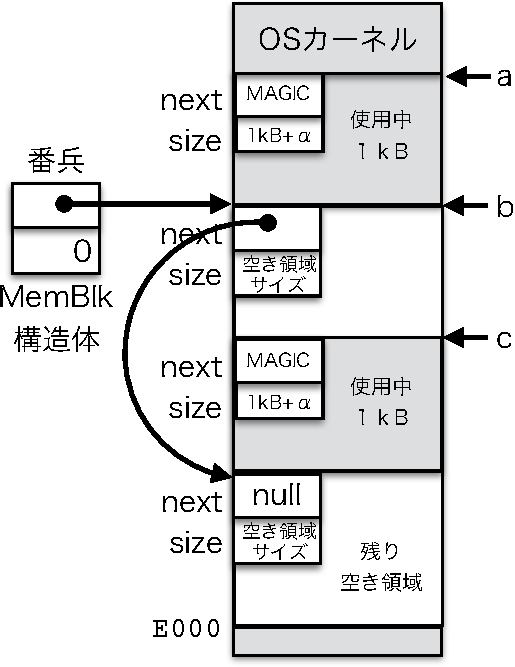
\includegraphics[scale=0.6]{Fig/mmFree1-crop.pdf}
    \end{center}
  \end{minipage}
  \begin{minipage}{0.49\columnwidth}
    \begin{center}
      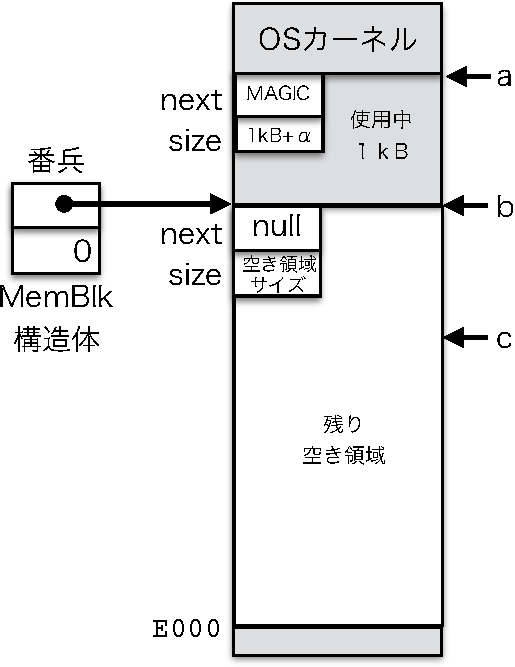
\includegraphics[scale=0.6]{Fig/mmFree2-crop.pdf}
    \end{center}
  \end{minipage}
\end{frame}

%=========================================================================
\begin{frame}
  \frametitle{メモリの解放プログラム(前半)}
  \lstinputlisting[lastline=15,frame=tlr]{Lst/mmFree.cmm}

  \begin{itemize}
  \item 領域の本当の先頭アドレスを計算する.
  \item {\tt MAGIC}を確認する.
  \item 空き領域リストを辿り,挿入位置を決める.
  \end{itemize}
\end{frame}

%=========================================================================
\begin{frame}
  \frametitle{メモリの解放プログラム}
  \lstinputlisting[firstline=16,frame=lrb]{Lst/mmFree.cmm}
\end{frame}

\end{document}

